\thesolution{Parco Pattini}
La struttura dati pu� essere realizzata come una lista dinamica semplicemente collegata in cui ogni elemento rappresenta lo stato di tutti i pattini di una data taglia. La generica cella della struttura contiene dunque:

\begin{itemize}
\item taglia dei pattini;
\item numero totale di pattini della taglia data;
\item numero totale di pattini disponibili della taglia data.
\end{itemize}
    
A titolo esemplificativo si immagini che il parco pattini disponga di un paio di pattini della taglia 44, di un paio della taglia 43 e di due paia della taglia 42. Se uno delle due paia di pattini della taglia 42 risulta fittato, lo stato della struttura � mostrato in \figurename~\ref{fig:Pattini}.
  
\begin{figure}
  \center
	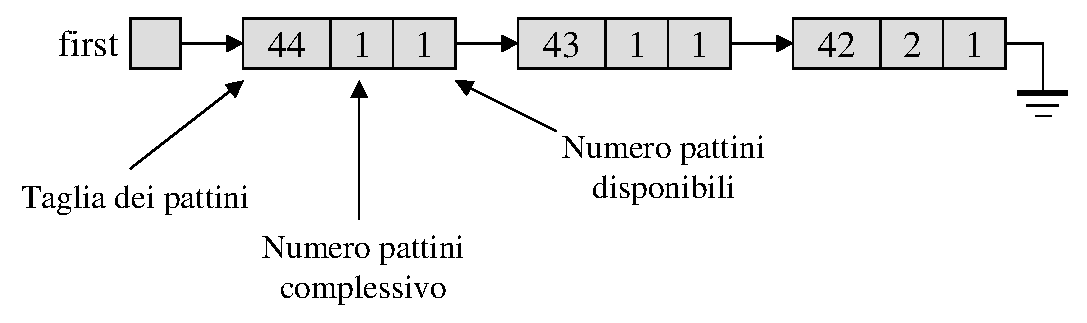
\includegraphics[width=.8\textwidth]{Esercizi/ParcoPattini/pattini.eps}
	\caption{La struttura che implementa il parco pattini.}
	\label{fig:Pattini}
\end{figure}

Si noti come la struttura ammetta una gestione di tipo tabellare, dal momento che la taglia dei pattini risulta essere unica per ogni cella, e quindi assimilabile ad una chiave.

Di seguito si riporta il listato.

\bigskip
\inputprogram{Esercizi/ParcoPattini/ParcoPattini.cpp}